
\section{Physics for derive $V_{cs}$ From $B(W\to l \nu)$ }
\label{sec:relatedWorks:vcs}





\subsection{NLO}


The coupling of W to lepton current is $g$ while to the quark current is $g|V_{ij}|$. 
\begin{equation}
    \feynmandiagram [inline=(d.base), small, horizontal=d to b] {
        a[particle=\(\nu_e\)] -- [fermion] b [dot] -- [fermion] c[particle=\(e^-\)],
        b -- [boson] d [particle=\(W^-\)],
    };
    = i g \gamma^{\mu} \qquad
    \feynmandiagram [inline=(d.base), small, horizontal=d to b] {
        a[particle=\(q_j\)] -- [fermion] b [dot] -- [fermion] c[particle=\(q_i\)],
        b -- [boson] d [particle=\(W^-\)],
    };
    = i g |V_{ij}|
\end{equation}

\noindent If we define the partial width of W to the lepton current $\Gamma_{W \to l \nu}$ as $\Gamma_l$, 
\begin{equation}
    \Gamma_l \equiv \Gamma_{W \to l \nu} =  \frac{g^2 m_W}{48 \pi} .
\end{equation}


\noindent  At tree-level, the W decay width to the quark current is
\begin{equation}
    \Gamma_{W \to q_i q_j}^{LO} = 3 |V_{ij}|^2 \frac{g^2 m_W}{48 \pi}  = 3 |V_{ij}|^2 \Gamma_l ,
\end{equation}

\noindent  where the factor 3 accounts for the three colors.
\begin{figure}
    \centering
    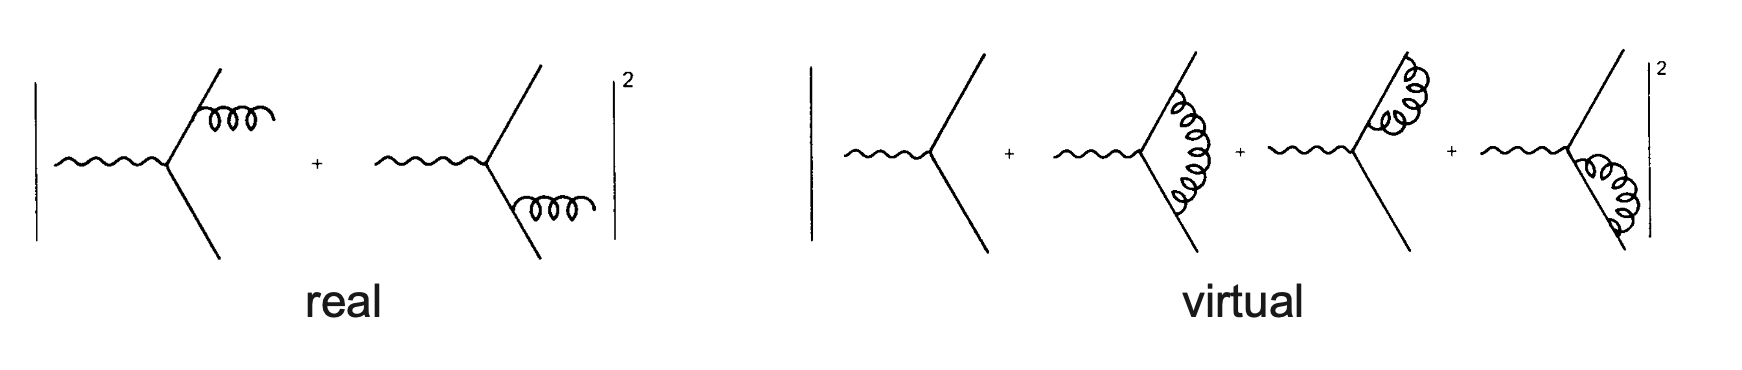
\includegraphics[width=0.8\textwidth]{chapters/RelatedWorks/sectionVcs/figures/realVirtual.png}
    \caption{ The real and virtual diagram of W decay considering the leading order QCD correction. }
    \label{fig:relatedWorks:vcs:realVirtual}
\end{figure}

\noindent However, at the NLO, QCD correction related to the quark current has to considered. More specifically, the real and virtual diagram, shown in Figure~\ref{fig:relatedWorks:vcs:realVirtual}, add extra contributions to the leading order width $\Gamma_{W \to q_i q_j}^{LO} $. The real diagram corresponds to the gluon final state radiation from the outcoming quarks. The virtual diagram corresponds to the interference between the tree level non-QCD process and the virtual gluon bubbles in the quark current and at the vertex. The calculation of the real and virtual contribution is usually expressed as a $k$ factor multiplied on the tree level rate  $\Gamma_{W \to q_i q_j}^{LO} $.
 \begin{align}
 	\Gamma^V_{W \to q_i q_j}  &= \Gamma_{W \to q_i q_j}^{LO} \times \frac{\alpha_s}{2\pi}\frac{4}{3} \bigg \{  -\ln^2\frac{m_g}{Q} -3 \ln\frac{m_g}{Q} + \frac{\pi^2}{3}-\frac{7}{2} \bigg\} \\
    \Gamma^R_{W \to q_i q_j}  &= \Gamma_{W \to q_i q_j}^{LO} \times \frac{\alpha_s}{2\pi}\frac{4}{3} \bigg \{  +\ln^2\frac{m_g}{Q} + 3 \ln\frac{m_g}{Q} - \frac{\pi^2}{3}+ 5 \bigg\}
\end{align}
 
\noindent  where $Q$ is the energy of W boson and $m_g$ is the mass of the massless gluon, which makes both the real and virtual width diverge. But the divergences in the real and virtual rate when $\lim m_g \to 0$ exactly cancel each other, producing a finite total contributions to the tree level width. This QCD correction turns out to be a $k$ factor of $1+\frac{\alpha_s}{\pi}$ :
\begin{equation}
\begin{split}
    \Gamma_{W \to q_i q_j}^{NLO} =& \Gamma_{W \to q_i q_j}^{LO} + \Gamma^{V}_{W \to q_i q_j}  + \Gamma^{R}_{W \to q_i q_j}
            =   \Gamma_{W \to q_i q_j}^{LO} \big( 1+ \frac{\alpha_s(M_W)}{\pi}\big)
%             =&  \Gamma_l \bigg[ 1+ \frac{\alpha_s(M_W)}{\pi} \bigg]  \sum_{color} \sum_{ i,j } |V_{ij}|^2  \\
%             =&  \Gamma_l \bigg[ 1+ \frac{ \alpha_s(\mu_R) - \alpha^2_s(\mu_R) \frac{ \beta_0}{2\pi} \ln \frac{M_W}{\mu_R}}{\pi} \bigg] \sum_{color} \sum_{ i,j } |V_{ij}|^2  
\end{split} .
\end{equation}

\noindent The factor of QCD contributions has been calculated with higher order corrections upto 3NLO. The state-of-art result of this factor reads 
\begin{equation}
	\rm{N^3LO:} \quad k = 1+1.045 ( \frac{\alpha_s}{\pi} ) + 0.94  ( \frac{\alpha_s}{\pi} ) ^2 -15  ( \frac{\alpha_s}{\pi} ) ^3.
\end{equation}
\noindent where $\alpha_s(M_W) = \alpha_s(\mu_R) - \alpha^2_s(\mu_R) \frac{ \beta_0}{2\pi} \ln \frac{M_W}{\mu_R}$ and the renormalization scale is conventionally chosen as Z mass $\mu_R=M_Z$. The running couplings derived from the higher order of QCD renormalization group equation is discussed in the Section~\ref{sec:relatedWorks:qft:qcd}. The latest PDG value of $\alpha_s(m_Z)=0.1178\pm0.0010$. Using the leading order running of coupling, the $\alpha_s$ at W pole is
\begin{equation}
	\alpha_s(M_W) = 0.1199 \pm 0.0010
\end{equation}
By definition, the branching fraction of W satisfies the unitary constrain
\begin{equation}
    \sum_{ i,j } B_{W \to q_i q_j} + 3 B_l = 1
\end{equation}

\noindent using  $B_{W \to q_i q_j} = 3 k |V_{ij}|^2 B_l $ to substitute $B_{W \to q_i q_j}$  with $B_l$, one gets
\begin{equation}
    \sum_{ i,j } |V_{ij}|^2 = \frac{1}{ 3k} \, \frac{1-3B_l}{B_l}
\end{equation}



\noindent  With $\sum_{ i,j } |V_{ij}|^2$ and the experimental value of other 5 better measured CKM elements \cite{pdg2020} in Table~\ref{tab:relatedWorks:vcs:ckm}, we can calculate the $V_{cs}$.



\subsection{higher order beyond NLO}
